\documentclass{article}

\author{Teddy Krulewich}
\title{\vspace{-4em}HW4 ME5501 – Robotics and Unmanned Systems}

\usepackage{graphicx}
\graphicspath{ {images/} }


\usepackage[utf8]{inputenc}
\usepackage{minted}
\usepackage{hyperref}
\usepackage{xcolor}
\definecolor{bg}{rgb}{0.95,0.95,0.95}
\usepackage{caption}
\usepackage{mdframed}

\begin{document}
\maketitle

\section*{Problem 1}
Complete the following ROS tutorials at \url{https://docs.ros.org/en/foxy/Tutorials.html}

• Understanding ROS Nodes

• Understanding ROS Topics

\bigskip
\noindent Save a screenshot of the Turtlebot simulator and show/print the screenshot.


\begin{figure}[H]
    \centering
    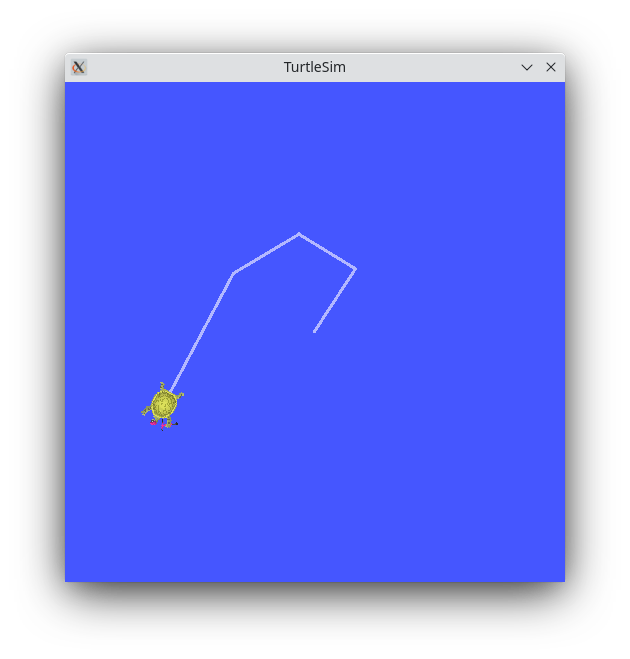
\includegraphics[width=0.5\textwidth]{question1.png}
    \caption*{Screenshot of Turtlebot Simulator}
\end{figure}

\section*{Problem 2}

Complete the following ROS tutorials at

\url{http://wiki.ros.org/ROS/Tutorials}


• 12. Writing a Simple Publisher and Subscriber (Python) 


• 13. Examining the Simple Publisher and Subscriber 

\bigskip 
\noindent Save a screenshot of the running code in tutorials 13, and print these screenshots to turn in.

\begin{figure}[H]
    \centering
    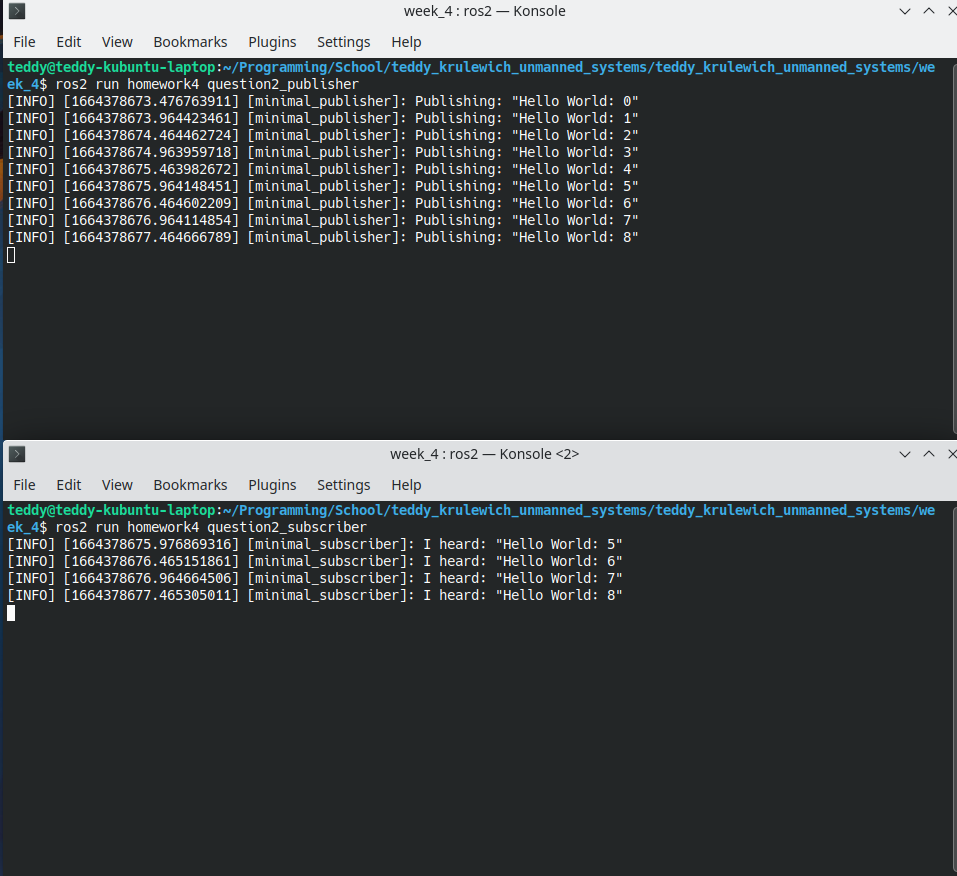
\includegraphics[width=\textwidth]{question2.png}
    \caption*{Screenshot of subscriber and publisher running}
\end{figure}

\end{document}